\documentclass{hmLab}

\usepackage{listings}
\usepackage[T1]{fontenc}
\usepackage[ngerman]{babel}
% These are some nice colors that fit well together
\definecolor{midnightblue}{RGB}{10,10,44}
\definecolor{navyblue}{RGB}{0,0,120}
\definecolor{crimson}{RGB}{220,20,60}
\definecolor{mydarkgray}{RGB}{33,33,33}
\definecolor{myalgColor}{RGB}{99,99,99}
\definecolor{mygreen}{RGB}{85,168,104}
\definecolor{myorange}{RGB}{221,132,82}
\definecolor{myblue2}{rgb}{0.12156862745098039, 0.4666666666666667, 0.7058823529411765}
\definecolor{myblue3}{rgb}{0.2980392156862745, 0.4470588235294118, 0.6901960784313725}
\definecolor{myblue4}{rgb}{0.2823529411764706, 0.47058823529411764, 0.8156862745098039}
\definecolor{mybluebright}{rgb}{0.00784313725490196, 0.24313725490196078, 1.0}
\definecolor{myred}{RGB}{196,78,82}
\definecolor{mydarkgray}{RGB}{90,90,90}
\definecolor{mygray}{RGB}{179,179,179}
\definecolor{myviolet}{RGB}{129,114,178}
\definecolor{myblue}{RGB}{76,114,202}
\xdefinecolor{mybg}{rgb}{0.7419607843137255, 0.9027297193387159, 0.868958093041138}
\xdefinecolor{myRed}{rgb}{0.7686274509803922, 0.3058823529411765, 0.3215686274509804}
\xdefinecolor{prevColor}{rgb}{0.39215686274509803, 0.7098039215686275, 0.803921568627451}
\xdefinecolor{mylightblue}{rgb}{0.8584083044982699, 0.9134486735870818, 0.9645674740484429}

\definecolor{mybrightblue}{rgb}{0.00784313725490196, 0.24313725490196078, 1.0}
\definecolor{mybrightred}{rgb}{0.9098039215686274, 0.0, 0.043137254901960784}

\xdefinecolor{myalgColor}{rgb}{0.7686274509803922, 0.3058823529411765, 0.3215686274509804}

% hm colors
\xdefinecolor{hmred}{RGB}{252, 85, 85}

%
\xdefinecolor{colordefinition}{RGB}{0, 123, 255}
\xdefinecolor{colorexample}{RGB}{200, 200, 200}

% listing colors
\definecolor{codegreen}{rgb}{0,0.6,0}
\definecolor{codegray}{rgb}{0.5,0.5,0.5}
\definecolor{codepurple}{rgb}{0.58,0,0.82}
\definecolor{backcolour}{rgb}{0.95,0.95,0.92}

\definecolor{halfgray}{gray}{0.55}
\definecolor{ipython_frame}{RGB}{207, 207, 207}
\definecolor{ipython_bg}{RGB}{247, 247, 247}
\definecolor{ipython_red}{RGB}{186, 33, 33}
\definecolor{ipython_green}{RGB}{0, 128, 0}
\definecolor{ipython_cyan}{RGB}{64, 128, 128}
\definecolor{ipython_purple}{RGB}{170, 34, 255}

\usepackage{courier}

\lstset{basicstyle=\footnotesize\ttfamily}
%\lstset{framextopmargin=50pt,frame=bottomline}

\lstdefinestyle{ipython}{
	commentstyle=\color{ipython_cyan}\ttfamily,
	stringstyle=\color{ipython_red}\ttfamily,
	keepspaces=true,
	showspaces=false,
	showstringspaces=false,
	%
	rulecolor=\color{ipython_frame},
	frame=single,
	frameround={t}{t}{t}{t},
	framexleftmargin=6mm,
	numbers=left,
	numberstyle=\tiny\color{halfgray},
	%
	%
	backgroundcolor=\color{ipython_bg},
	%   extendedchars=true,
	basicstyle=\scriptsize\ttfamily\scriptsize,
	keywordstyle=\color{ipython_green}\bfseries,
	%backgroundcolor=\color{backcolour},   
	breakatwhitespace=false,         
	breaklines=true,                 
	captionpos=b,                    
	keepspaces=true,                 
	numbers=left,                    
	numbersep=5pt,                            
	showtabs=false,                  
	tabsize=2
}

\lstdefinelanguage{opencl}
{morekeywords={const,double,int,if,get_global_id,unsigned,__kernel,kernel,__local,local,__global,global,% 
		__constant,constant,__private,private,% 
		char2,char3,char4,char8,char16,% 
		uchar2,uchar3,uchar4,uchar8,uchar16,% 
		short2,short3,short4,short8,short16,% 
		ushort2,ushort3,ushort4,ushort8,ushort16,% 
		int2,int3,int4,int8,int16,% 
		uint2,uint3,uint4,uint8,uint16,% 
		long2,long3,long4,long8,long16,% 
		ulong2,ulong3,ulong4,ulong8,ulong16,% 
		float2,float3,float4,float8,float16,% 
		image2d_t,image3d_t,sampler_t,event_t,% 
		bool2,bool3,bool4,bool8,bool16,% 
		half2,half3,half4,half8,half16,% 
		quad,quad2,quad3,quad4,quad8,quad16,% 
		complex,imaginary},% 
}% 

\lstdefinestyle{mystyle}{
	%backgroundcolor=\color{backcolour},   
	commentstyle=\color{codegreen},
	keywordstyle=\color{magenta},
	numberstyle=\tiny\color{codegray},
	stringstyle=\color{codepurple},
	basicstyle=\ttfamily\footnotesize\scriptsize,
	breakatwhitespace=false,         
	breaklines=true,                 
	captionpos=b,                    
	keepspaces=true,                 
	numbers=left,                    
	numbersep=5pt,                  
	showspaces=false,                
	showstringspaces=false,
	showtabs=false,                  
	tabsize=2
}

\usepackage{color}
\definecolor{lightgray}{rgb}{.9,.9,.9}
\definecolor{darkgray}{rgb}{.4,.4,.4}
\definecolor{purple}{rgb}{0.65, 0.12, 0.82}
\definecolor{pink}{RGB}{201, 28, 164}
\lstdefinelanguage{p5js}{
	keywords={constructor, console, log, class, export, boolean, throw, implements, import, this, let,var,break, case, catch, continue, debugger, default, delete, do, else, false, finally, for, function, if, in, instanceof, new, null, return, switch, this, throw, true, try, typeof, var, void, while, with},
	morecomment=[l]{//},
	morecomment=[s]{/*}{*/},
	morestring=[b]',
	morestring=[b]",
	ndkeywords={setup, push, pop, rotate, scale, translate, draw, width, height, createCanvas, background, stroke, fill, rect, line,curve,random},
	keywordstyle=\color{blue}\bfseries,
	ndkeywordstyle=\color{pink}\bfseries,
	identifierstyle=\color{black},
	commentstyle=\color{purple}\ttfamily,
	stringstyle=\color{ipython_red}\ttfamily,
	sensitive=true
}

\lstset{style=ipython}


\course{Computational Thinking}
\semester{WS2023/24}
\labno{2}
\subtitle{Kontrollstrukturen mit dem micro:bit}
\author{Prof.\,Dr.-Ing.\,Martin Hobelsberger\\Dr.\,Benedikt Zönnchen\\Prof.\,Dr.-Ing.\,Benedikt Dietrich}

\begin{document}
\maketitle

\section*{Lernziel}

In dieser ersten praktischen Übung konzentrieren wir uns aufs Denken.
Nach diesem Praktikum sollten Sie die Fähigkeiten haben:

\begin{enumerate}[label=$\bullet$]
	\item einfache Problemstellungen zu analysieren, diese zu verstehen und in (kleinste) Teilprobleme untergliedern/strukturieren können 
	\item für Teilprobleme eine abstrakte Lösung zu überlegen und diese in eigenen Worten niederzuschreiben 
	\item einfache logischen Einheiten der Programmierung (z.B. Schleifen und Variablen) nachvollziehen zu können und diese auf eine abstrakte Lösung anzuwenden
\end{enumerate}

\section*{Voraussetzungen}

Wir verwenden das \textit{micro:bit} (einen sog. Einplatinencomputer), welches unsere Algorithmen ausführt.
Sie können die Algorithmen auch ohne das \textit{micro:bit} entwickeln und testen, doch wollen wir diese dann auch auf dem \textit{micro:bit} ausführen um diesen Computer zu steuern.
Im Praktikum erhalten Sie ein \textit{micro:bit} pro Gruppe.
Testen Sie alle Lösungen auf Ihrem \textit{micro:bit}!

\newpage

\excercise{Einführung und Tutorial}

Bevor Sie mit der abzugebenden Aufgabe beginnen sollten Sie sich mit der Entwicklungsumgebung vertraut machen. 
Gehen Sie hierzu wie folgt vor:

\begin{enumerate}[label=(\arabic*)]
	\item Lesen Sie sich folgende Anleitung durch: \href{http://microbit.org/de/guide/quick/}{http://microbit.org/de/guide/quick/}
	\item Folgen Sie zum Lösen der Aufgaben den notwendigen Schritten (unter Verwendung der Umgebung unter: \href{https://makecode.microbit.org/}{https://makecode.microbit.org/})
\end{enumerate}
%
Versuchen Sie nun verschiedene kleine Aufgaben zu lösen.
Verwenden Sie hier logische Einheiten aus den Reitern Grundlagen und Eingabe:

\begin{figure}[h!]
	\centering
	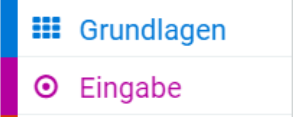
\includegraphics[width=0.3\textwidth]{basics-input}
\end{figure}

\begin{enumerate}[label=$\bullet$]
	\item Geben Sie ``Hallo Welt!'' oder Ihren Namen auf dem Display (LED-Matrix) aus.
	\begin{figure}[h!]
		\centering
		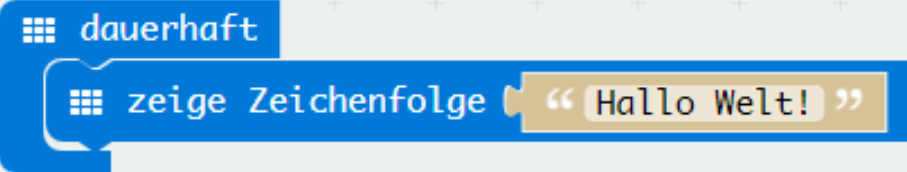
\includegraphics[width=0.6\textwidth]{hello-world}
	\end{figure}
	\item Zeichnen Sie, auf Knopfdruck (A oder B) kleine Bilder auf den Bildschirm 
	\begin{figure}[h!]
		\centering
		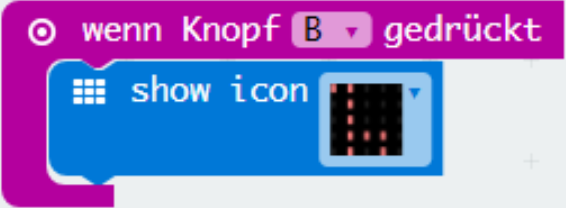
\includegraphics[width=0.4\textwidth]{a-or-b}
	\end{figure}
	\item Zeigen Sie nach Start eine Zahl an und löschen Sie diese nach der Anzeige wieder.
	\begin{figure}[h!]
		\centering
		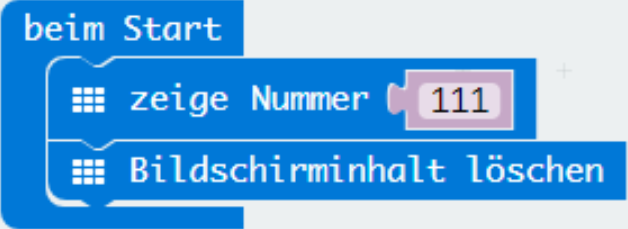
\includegraphics[width=0.4\textwidth]{show-number}
	\end{figure}
	\item Überlegen Sie sich mit Ihrem Gruppenpartner eigene kleine Aufgaben die Sie sich gegenseitig stellen! Fordern Sie sich gegenseitig heraus!
\end{enumerate}

\excercise{Schleifen: X}

Implementieren Sie einen Algorithmus um durch drücken der \textbf{Taste\,A} und der \textbf{Taste\,B} ein X auf den Bildschirm zu zeichnen.\\

\noindent In dieser Aufgabe lernen Sie die Grundzüge der Verwendung von Schleifen (Befehle mehrmals ausführen) und Variablen (Daten zwischenspeichern).
Am Ende dieser Aufgabe haben Sie ein Programm entwickelt das folgende Funktion erfüllt:
%
\begin{figure}[h!]
	\centering
	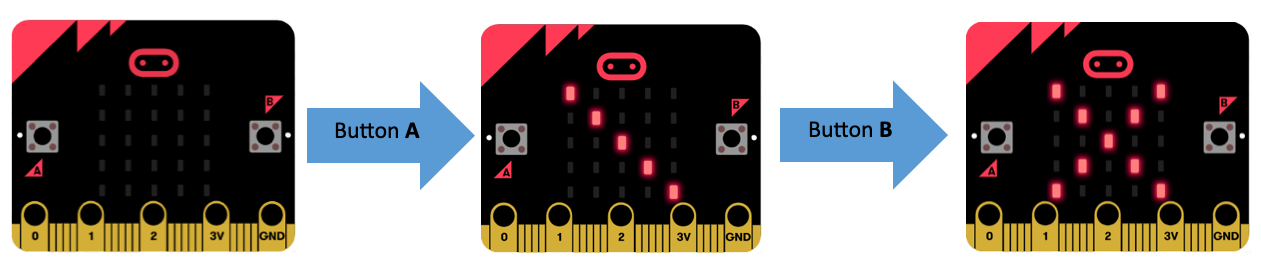
\includegraphics[width=0.8\textwidth]{microbit-X}
\end{figure}
%
Verwenden Sie hierzu \textbf{NUR} logische Elemente aus der Kategorie:
%
\begin{enumerate}[label=$\bullet$]
	\item Eingabe 
	\begin{figure}[h!]
		\centering
		
\includegraphics[width=0.2\textwidth]{input}
	\end{figure}
	\item LED
	\begin{figure}[h!]
		\centering
		
\includegraphics[width=0.2\textwidth]{led}
	\end{figure}
	\item Schleifen
	\begin{figure}[h!]
		\centering
		
\includegraphics[width=0.2\textwidth]{loop}
	\end{figure}
	\item Variablen
	\begin{figure}[h!]
		\centering
		
\includegraphics[width=0.21\textwidth]{variables}
	\end{figure}
\end{enumerate}

Gehen Sie dazu wie folgt vor:
\begin{enumerate}[label=\arabic*.]
	\item Versuchen Sie das Problem in Teilprobleme zu zerlegen. Überlegen Sie sich, z.\,B., zuerst den Algorithmus für \textbf{Taste\,A} und dann für \textbf{Taste\,B}.
	Wie würden Sie vorgehen, wenn Sie auf einem Blatt Papier die einzelnen LEDs ($5 \times 5$ an der Zahl) im vorgegebenen Muster ausmalen müssten? 
	Schreiben Sie die einzelnen Schritte auf!\\\\\textbf{Tipp}: Die \textbf{LEDs} sind in einer Matrix ($x$- und $y$-Koordinaten) angeordnet und können auch so bedient werden: 
	Die \textbf{LED} in der linken oberen Ecke ist mit den Koordinaten $(0,0)$ also $x$ entspricht 0 und $y$ entspricht 0 beschrieben.
	Die \textbf{LED} in der rechten unteren Ecke hat die Koordinaten $(4,4)$.
	\item Machen Sie sich mit den einzelnen logischen Elementen in den Kategorien vertraut! Versuchen Sie für jedes einzelne Element ein kleines Programm zu erstellen um die Funktion kennen zu lernen. 
	\item Wählen Sie die logischen Elemente aus welche Sie für Ihre Lösung am geeignetsten halten und versuchen Sie das Programm in Teilschritten zu erstellen. Nutzen Sie immer wieder den Simulator um Ihr Programm zu überprüfen! 
\end{enumerate}

\excercise{Treppenbau}

Zeichnen Sie, durch mehrmaliges drücken von \textbf{Taste A}, eine Treppe wie diese in folgender Abbildung dargestellt wird.
%
\begin{figure}[h!]
	\centering
	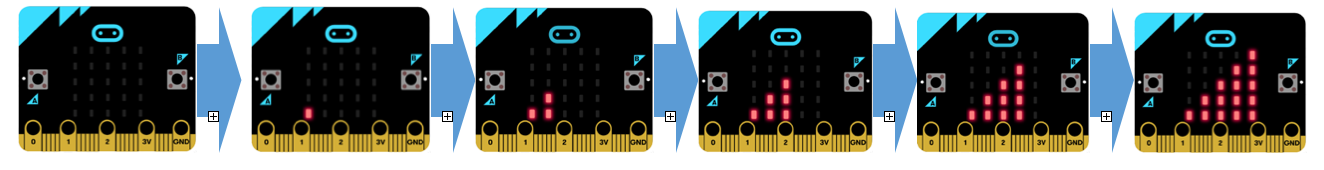
\includegraphics[width=1.0\textwidth]{stairs}
\end{figure}
%
Auch hier verwenden Sie \textbf{NUR} wieder die logischen Elemente aus Eingabe, LED, Schleifen und Variablen. 

\excercise{Treppenbau}

Und noch etwas kniffliger. Zeichnen Sie, durch mehrmaliges drücken von \textbf{Taste B}, eine Treppe mit einem Absatz! 
%
\begin{figure}[h!]
	\centering
	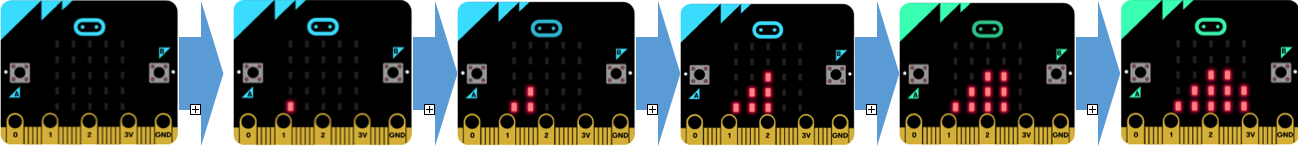
\includegraphics[width=1.0\textwidth]{stairs-with-floor}
\end{figure}
%
Auch hier verwenden Sie \textbf{NUR} wieder die logischen Elemente aus Eingabe, LED, Schleifen, Variablen und \textbf{ZUSÄTZLICH} aus der Kategorie Logik
	\begin{figure}[h!]
	\centering
	
\includegraphics[width=0.2\textwidth]{logic}
\end{figure}


\section*{Weiterführende Informationen}

\begin{enumerate}[label=$\bullet$]
	\item \href{http://microbit.org/de/ideas/}{http://microbit.org/de/ideas/}
	\item \href{https://makecode.com/\#get-inspired}{https://makecode.com/\#get-inspired}
\end{enumerate}

\end{document}
